% Chapter 10: Use Cases
\chapter{Use Cases}
\label{ch:use-cases}

\tprotocol{} enables diverse payment scenarios across web services, AI agents, digital content, and IoT devices. This chapter explores practical applications with detailed implementation patterns.

\section{AI Agent Payments}
\label{sec:ai-payments}

The emergence of autonomous AI agents creates unprecedented demand for machine-to-machine payments. Unlike humans, AI agents cannot use traditional payment methods that require manual intervention.

\subsection{The Agent Payment Problem}

\begin{figure}[ht]
\centering
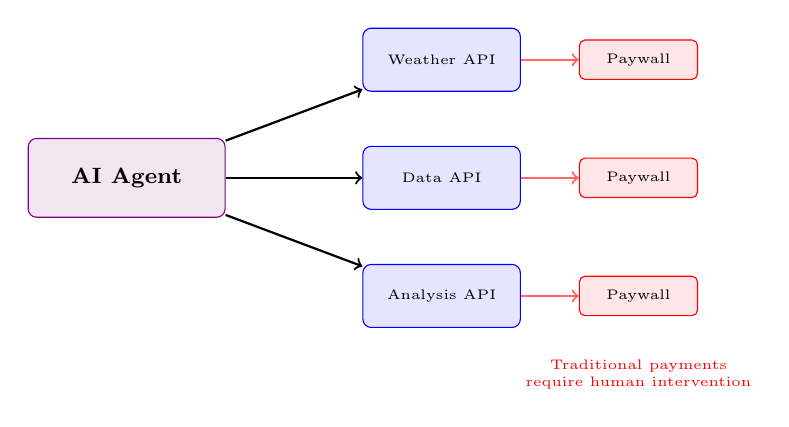
\begin{tikzpicture}[
    agent/.style={
        rectangle,
        rounded corners=3pt,
        minimum width=2.5cm,
        minimum height=1cm,
        draw=violet,
        fill=violet!10,
        font=\footnotesize\bfseries,
        align=center
    },
    service/.style={
        rectangle,
        rounded corners=3pt,
        minimum width=2cm,
        minimum height=0.8cm,
        draw=blue,
        fill=blue!10,
        font=\tiny,
        align=center
    },
    block/.style={
        rectangle,
        rounded corners=2pt,
        minimum width=1.5cm,
        minimum height=0.5cm,
        draw=red,
        fill=red!10,
        font=\tiny
    }
]

\node[agent] (agent) at (0,0) {AI Agent};

\node[service] (api1) at (4,1.5) {Weather API};
\node[service] (api2) at (4,0) {Data API};
\node[service] (api3) at (4,-1.5) {Analysis API};

\node[block] (pay1) at (6.5,1.5) {Paywall};
\node[block] (pay2) at (6.5,0) {Paywall};
\node[block] (pay3) at (6.5,-1.5) {Paywall};

% Arrows
\draw[->, thick] (agent) -- (api1);
\draw[->, thick] (agent) -- (api2);
\draw[->, thick] (agent) -- (api3);

\draw[->, thick, red!60] (api1) -- (pay1);
\draw[->, thick, red!60] (api2) -- (pay2);
\draw[->, thick, red!60] (api3) -- (pay3);

% Problem annotation
\node[font=\tiny, red, align=center] at (6.5,-2.5) {Traditional payments\\require human intervention};

\end{tikzpicture}
\caption{AI agents blocked by traditional paywalls}
\label{fig:agent-problem}
\end{figure}

AI agents require:

\begin{table}[ht]
\centering
\caption{AI Agent Payment Requirements}
\label{tab:agent-requirements}
\begin{tabular}{l p{6.5cm}}
\toprule
\textbf{Requirement} & \textbf{Description} \\
\midrule
Programmatic Access & No UI interaction, pure API \\
Budget Control & Configurable spending limits \\
Cost Visibility & Know price before execution \\
Autonomous Execution & No human approval per transaction \\
Failure Handling & Graceful degradation on payment failure \\
\bottomrule
\end{tabular}
\end{table}

\subsection{MCP Tool Marketplace}

The Model Context Protocol enables AI agents to discover and use paid tools:

\begin{lstlisting}[language=typescript,caption={AI agent with budget management}]
import { Agent } from "@langchain/core";
import { T402McpClient } from "@t402/mcp-client";

const mcpClient = new T402McpClient({
  signer: agentWallet,
  budget: {
    maxPerCall: "100000",    // $0.10 max per call
    maxPerHour: "1000000",   // $1.00 max per hour
    maxPerDay: "10000000"    // $10.00 max per day
  },
  onBudgetExceeded: async (cost) => {
    // Notify operator
    await alertOperator(`Budget exceeded: ${cost}`);
    return false;  // Reject payment
  }
});

// Agent discovers available tools
const tools = await mcpClient.listTools();
// Returns: [
//   { name: "stock_analysis", price: "$0.10" },
//   { name: "sentiment_analysis", price: "$0.05" },
//   { name: "market_report", price: "$0.50" }
// ]

// Agent evaluates cost vs value
const agent = new Agent({
  tools: tools.filter(t =>
    parseFloat(t.price.slice(1)) <= 0.10
  ),
  mcpClient
});

// Execute task with automatic payments
const result = await agent.run(
  "Analyze AAPL stock sentiment from recent news"
);
\end{lstlisting}

\subsection{Agent-to-Agent Economy}

\begin{figure}[ht]
\centering
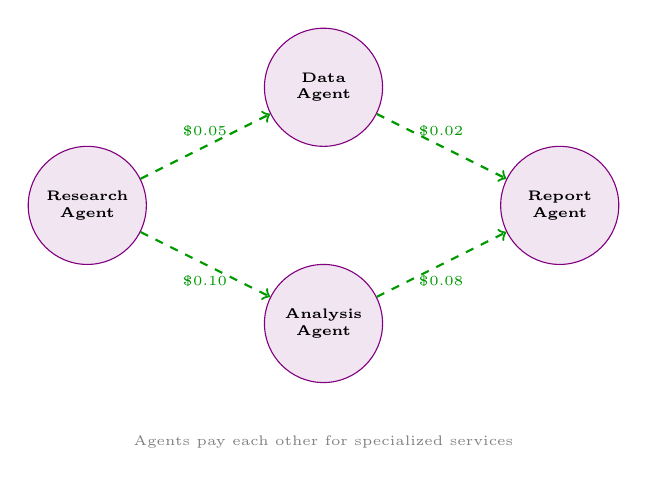
\begin{tikzpicture}[
    agent/.style={
        circle,
        minimum size=1.5cm,
        draw=violet,
        fill=violet!10,
        font=\tiny\bfseries,
        align=center
    },
    payment/.style={
        ->,
        thick,
        green!60!black,
        dashed
    }
]

\node[agent] (a1) at (0,0) {Research\\Agent};
\node[agent] (a2) at (3,1.5) {Data\\Agent};
\node[agent] (a3) at (3,-1.5) {Analysis\\Agent};
\node[agent] (a4) at (6,0) {Report\\Agent};

\draw[payment] (a1) -- node[above, font=\tiny] {\$0.05} (a2);
\draw[payment] (a1) -- node[below, font=\tiny] {\$0.10} (a3);
\draw[payment] (a2) -- node[above, font=\tiny] {\$0.02} (a4);
\draw[payment] (a3) -- node[below, font=\tiny] {\$0.08} (a4);

\node[font=\tiny, gray] at (3,-3) {Agents pay each other for specialized services};

\end{tikzpicture}
\caption{Agent-to-agent payment flows}
\label{fig:a2a-economy}
\end{figure}

\section{API Monetization}
\label{sec:api-monetization}

Transform any REST API into a paid service with per-request billing.

\subsection{Traditional vs T402 Monetization}

\begin{table}[ht]
\centering
\caption{API Monetization Comparison}
\label{tab:monetization-comparison}
\footnotesize
\begin{tabular}{l p{4cm} p{4cm}}
\toprule
\textbf{Aspect} & \textbf{Traditional (Stripe)} & \textbf{T402} \\
\midrule
Setup & Create plans, pricing tiers & Add middleware \\
User Flow & Sign up $\to$ Subscribe $\to$ Use & Use $\to$ Pay $\to$ Access \\
Billing & Monthly invoices & Per-request instant \\
Minimum & \$5-10/month subscription & \$0.001 per call \\
Global & Credit card regions & Worldwide (crypto) \\
Settlement & 2-3 business days & Instant \\
\bottomrule
\end{tabular}
\end{table}

\subsection{Weather Data API Example}

\begin{lstlisting}[language=typescript,caption={Weather API with tiered pricing}]
import express from "express";
import { paymentMiddleware } from "@t402/express";

const app = express();

// Tiered pricing based on data resolution
const pricingTiers = {
  "GET /api/weather/current": {
    price: "$0.001",
    description: "Current weather"
  },
  "GET /api/weather/forecast/hourly": {
    price: "$0.005",
    description: "48-hour hourly forecast"
  },
  "GET /api/weather/forecast/daily": {
    price: "$0.01",
    description: "14-day daily forecast"
  },
  "GET /api/weather/historical": {
    price: async (req) => {
      // Price based on date range
      const days = calculateDays(req.query.start, req.query.end);
      return `$${(days * 0.001).toFixed(4)}`;
    },
    description: "Historical weather data"
  }
};

app.use(paymentMiddleware({
  routes: pricingTiers,
  payTo: "0xWeatherServiceWallet..."
}));

// Endpoints
app.get("/api/weather/current", async (req, res) => {
  const { lat, lon } = req.query;
  const weather = await getWeather(lat, lon);
  res.json(weather);
});
\end{lstlisting}

\subsection{Revenue Dashboard}

\begin{figure}[ht]
\centering
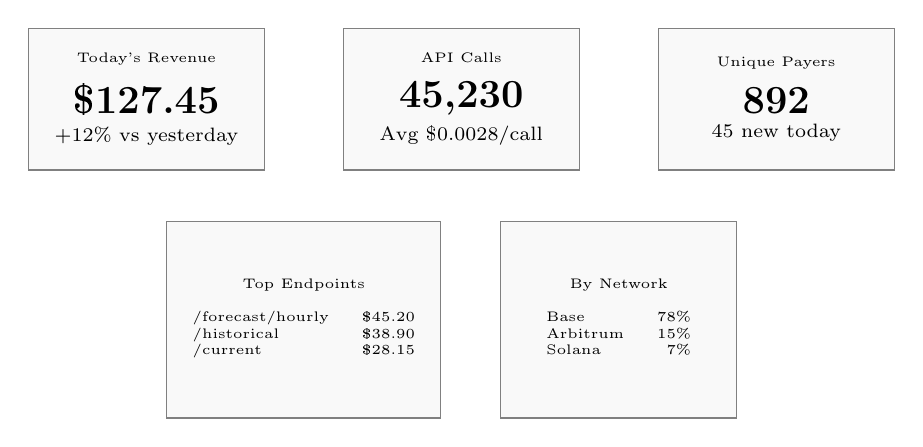
\begin{tikzpicture}[
    panel/.style={
        rectangle,
        minimum width=3cm,
        minimum height=1.8cm,
        draw=gray,
        fill=gray!5,
        font=\tiny,
        align=center
    }
]

\node[panel] at (0,0) {Today's Revenue\\[0.2cm]\Large\bfseries \$127.45\\[0.1cm]\scriptsize +12\% vs yesterday};
\node[panel] at (4,0) {API Calls\\[0.2cm]\Large\bfseries 45,230\\[0.1cm]\scriptsize Avg \$0.0028/call};
\node[panel] at (8,0) {Unique Payers\\[0.2cm]\Large\bfseries 892\\[0.1cm]\scriptsize 45 new today};

\node[panel, minimum height=2.5cm] at (2,-2.8) {
    Top Endpoints\\[0.2cm]
    \begin{tabular}{lr}
    /forecast/hourly & \$45.20 \\
    /historical & \$38.90 \\
    /current & \$28.15 \\
    \end{tabular}
};

\node[panel, minimum height=2.5cm] at (6,-2.8) {
    By Network\\[0.2cm]
    \begin{tabular}{lr}
    Base & 78\% \\
    Arbitrum & 15\% \\
    Solana & 7\% \\
    \end{tabular}
};

\end{tikzpicture}
\caption{API monetization dashboard}
\label{fig:api-dashboard}
\end{figure}

\section{Content Access}
\label{sec:content-access}

Enable pay-per-article, pay-per-video, and premium content access without subscriptions.

\subsection{The Subscription Fatigue Problem}

\begin{infobox}[Subscription Fatigue]
The average consumer subscribes to 6+ content services at \$10-15/month each. Most content goes unconsumed. \tprotocol{} enables pay-per-use: read one article for \$0.25 instead of subscribing for \$10/month.
\end{infobox}

\subsection{News Article Paywall}

\begin{lstlisting}[language=typescript,caption={News paywall implementation}]
// Next.js API route with T402
import { withPayment } from "@t402/next";

export default withPayment(
  async function handler(req, res) {
    const { slug } = req.query;
    const article = await getArticle(slug);

    res.json({
      title: article.title,
      content: article.content,
      author: article.author
    });
  },
  {
    // Dynamic pricing by article type
    price: async (req) => {
      const article = await getArticleMeta(req.query.slug);
      const prices = {
        "breaking": "0.10",
        "analysis": "0.25",
        "research": "0.50",
        "standard": "0.05"
      };
      return prices[article.type] || "0.10";
    },
    network: "eip155:8453"
  }
);
\end{lstlisting}

\subsection{Video Streaming}

\begin{lstlisting}[language=typescript,caption={Pay-per-view video streaming}]
// Video access with time-based pricing
app.get("/api/video/:id/access",
  paymentMiddleware.route({
    price: async (req) => {
      const video = await getVideoMeta(req.params.id);
      // $0.01 per minute of content
      return `$${(video.duration / 60 * 0.01).toFixed(4)}`;
    }
  }),
  async (req, res) => {
    const { payer, transaction } = req.t402Payment;

    // Generate time-limited access token
    const accessToken = await generateAccessToken({
      videoId: req.params.id,
      payer,
      transaction,
      expiresIn: "24h"
    });

    res.json({
      accessToken,
      streamUrl: `/stream/${req.params.id}?token=${accessToken}`
    });
  }
);
\end{lstlisting}

\section{Micropayments}
\label{sec:micropayments}

Enable payments below traditional minimums (\$0.50) for IoT, compute, and data services.

\subsection{Economic Viability}

\begin{table}[ht]
\centering
\caption{Micropayment Economics}
\label{tab:micropayment-economics}
\footnotesize
\begin{tabular}{l r r r}
\toprule
\textbf{Payment} & \textbf{Stripe Fee} & \textbf{T402 Fee} & \textbf{Savings} \\
\midrule
\$0.01 & \$0.30 (3000\%) & \$0.0001 (1\%) & 99.97\% \\
\$0.10 & \$0.33 (330\%) & \$0.001 (1\%) & 99.70\% \\
\$1.00 & \$0.33 (33\%) & \$0.01 (1\%) & 97.0\% \\
\$10.00 & \$0.59 (5.9\%) & \$0.10 (1\%) & 83.1\% \\
\bottomrule
\end{tabular}
\end{table}

\subsection{IoT Data Marketplace}

\begin{lstlisting}[language=typescript,caption={IoT sensor data marketplace}]
// Sensor data pricing: $0.0001 per reading
const sensorPricing = {
  temperature: "0.0001",
  humidity: "0.0001",
  air_quality: "0.0005",
  traffic: "0.001",
  energy: "0.0002"
};

app.get("/api/sensors/:type/latest",
  paymentMiddleware.route({
    price: (req) => sensorPricing[req.params.type] || "0.001"
  }),
  async (req, res) => {
    const reading = await getSensorReading(req.params.type);
    res.json(reading);
  }
);

// Bulk data: $0.05 per 1000 readings
app.get("/api/sensors/:type/bulk",
  paymentMiddleware.route({
    price: async (req) => {
      const count = Math.min(req.query.count || 100, 10000);
      const basePrice = parseFloat(sensorPricing[req.params.type]);
      return `$${(count * basePrice * 0.8).toFixed(6)}`;  // 20% bulk discount
    }
  }),
  async (req, res) => {
    const readings = await getBulkReadings(
      req.params.type,
      req.query.count
    );
    res.json(readings);
  }
);
\end{lstlisting}

\subsection{Compute-on-Demand}

\begin{figure}[ht]
\centering
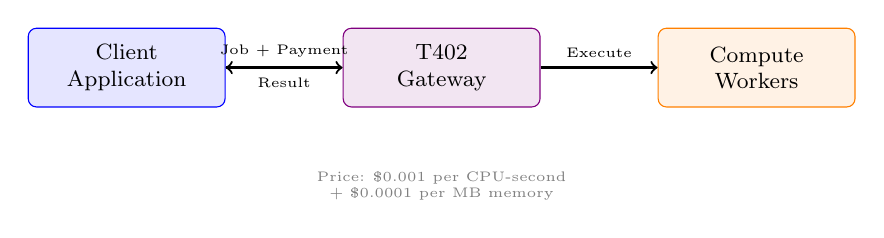
\begin{tikzpicture}[
    node/.style={
        rectangle,
        rounded corners=3pt,
        minimum width=2.5cm,
        minimum height=1cm,
        draw=blue,
        fill=blue!10,
        font=\footnotesize,
        align=center
    }
]

\node[node] (client) at (0,0) {Client\\Application};
\node[node, draw=violet, fill=violet!10] (gateway) at (4,0) {T402\\Gateway};
\node[node, draw=orange, fill=orange!10] (compute) at (8,0) {Compute\\Workers};

\draw[->, thick] (client) -- node[above, font=\tiny] {Job + Payment} (gateway);
\draw[->, thick] (gateway) -- node[above, font=\tiny] {Execute} (compute);
\draw[<-, thick, dashed] (client) -- node[below, font=\tiny] {Result} (gateway);

\node[font=\tiny, gray, align=center] at (4,-1.5) {Price: \$0.001 per CPU-second\\+ \$0.0001 per MB memory};

\end{tikzpicture}
\caption{Pay-per-compute architecture}
\label{fig:compute-architecture}
\end{figure}

\begin{lstlisting}[language=typescript,caption={Serverless compute pricing}]
// Price based on estimated compute resources
app.post("/api/compute/run",
  paymentMiddleware.route({
    price: async (req) => {
      const { code, timeout, memory } = req.body;

      // Estimate cost
      const cpuSeconds = timeout / 1000;
      const memoryMB = memory / (1024 * 1024);

      const cpuCost = cpuSeconds * 0.001;    // $0.001/CPU-sec
      const memoryCost = memoryMB * 0.0001;  // $0.0001/MB

      return `$${(cpuCost + memoryCost).toFixed(6)}`;
    }
  }),
  async (req, res) => {
    const result = await executeInSandbox(req.body);
    res.json({
      result: result.output,
      metrics: {
        cpuTime: result.cpuTime,
        memoryUsed: result.memoryUsed
      }
    });
  }
);
\end{lstlisting}

\section{Cross-Border Payments}
\label{sec:cross-border}

Enable instant global payments without currency conversion or banking restrictions.

\subsection{Traditional Cross-Border Challenges}

\begin{table}[ht]
\centering
\caption{Cross-Border Payment Comparison}
\label{tab:cross-border}
\footnotesize
\begin{tabular}{l l l l}
\toprule
\textbf{Method} & \textbf{Time} & \textbf{Fee} & \textbf{Access} \\
\midrule
Wire Transfer & 3-5 days & \$25-50 & Bank account \\
PayPal & 1-3 days & 4-5\% & Limited countries \\
Stripe & 2-7 days & 3.9\% + \$0.30 & Credit card \\
T402 & Instant & $<$1\% & Global (crypto wallet) \\
\bottomrule
\end{tabular}
\end{table}

\subsection{Freelancer Platform}

\begin{lstlisting}[language=typescript,caption={Global freelancer payments}]
// Freelancer delivers work, client pays instantly
app.post("/api/deliverables/:id/accept",
  paymentMiddleware.route({
    price: async (req) => {
      const deliverable = await getDeliverable(req.params.id);
      return deliverable.agreedPrice;
    },
    payTo: async (req) => {
      // Pay directly to freelancer's wallet
      const deliverable = await getDeliverable(req.params.id);
      return deliverable.freelancerWallet;
    }
  }),
  async (req, res) => {
    const { transaction } = req.t402Payment;

    // Mark as paid
    await updateDeliverable(req.params.id, {
      status: "paid",
      paymentTx: transaction
    });

    // Release to client
    const deliverable = await getDeliverable(req.params.id);
    res.json({
      files: deliverable.files,
      paymentConfirmation: transaction
    });
  }
);
\end{lstlisting}

\section{Research Data Access}
\label{sec:research-data}

Academic and commercial research data marketplaces.

\begin{lstlisting}[language=typescript,caption={Research dataset marketplace}]
// Dataset pricing tiers
const datasetPricing = {
  preview: { rows: 100, price: "0" },
  sample: { rows: 1000, price: "1.00" },
  standard: { rows: 10000, price: "5.00" },
  full: { rows: -1, price: "25.00" }  // Unlimited
};

app.get("/api/datasets/:id/download",
  paymentMiddleware.route({
    price: (req) => {
      const tier = req.query.tier || "sample";
      return datasetPricing[tier]?.price || "5.00";
    },
    // Free preview tier
    skipPayment: (req) => req.query.tier === "preview"
  }),
  async (req, res) => {
    const tier = req.query.tier || "sample";
    const dataset = await getDataset(req.params.id);
    const limit = datasetPricing[tier].rows;

    const data = limit === -1
      ? dataset.data
      : dataset.data.slice(0, limit);

    res.json({
      metadata: dataset.metadata,
      data,
      tier,
      totalRows: dataset.data.length
    });
  }
);
\end{lstlisting}

\section{Gaming and Virtual Goods}
\label{sec:gaming}

In-game purchases and virtual item trading.

\begin{lstlisting}[language=typescript,caption={Game item marketplace}]
// In-game item purchase
app.post("/api/game/items/purchase",
  paymentMiddleware.route({
    price: async (req) => {
      const item = await getGameItem(req.body.itemId);
      return item.price;
    }
  }),
  async (req, res) => {
    const { payer, transaction } = req.t402Payment;
    const { itemId, playerId } = req.body;

    // Grant item to player
    await grantItem(playerId, itemId, {
      purchasedBy: payer,
      transaction
    });

    res.json({
      success: true,
      item: await getPlayerInventory(playerId, itemId)
    });
  }
);

// Player-to-player trading
app.post("/api/game/trade/execute",
  paymentMiddleware.route({
    price: (req) => req.body.price,
    payTo: async (req) => {
      // Pay seller directly
      const seller = await getPlayer(req.body.sellerId);
      return seller.walletAddress;
    }
  }),
  async (req, res) => {
    // Transfer item between players
    await transferItem(
      req.body.sellerId,
      req.body.buyerId,
      req.body.itemId
    );

    res.json({ success: true });
  }
);
\end{lstlisting}

\section{Decision Framework}
\label{sec:decision-framework}

Use this framework to determine if \tprotocol{} is appropriate for your use case.

\begin{figure}[ht]
\centering
\begin{tikzpicture}[
    decision/.style={
        diamond,
        aspect=2.5,
        draw=violet,
        fill=violet!10,
        font=\tiny,
        align=center
    },
    outcome/.style={
        rectangle,
        rounded corners=3pt,
        draw=green!60!black,
        fill=green!10,
        minimum width=2cm,
        minimum height=0.6cm,
        font=\tiny,
        align=center
    },
    negative/.style={
        rectangle,
        rounded corners=3pt,
        draw=red,
        fill=red!10,
        minimum width=2cm,
        minimum height=0.6cm,
        font=\tiny,
        align=center
    },
    arrow/.style={->, thick}
]

\node[decision] (start) at (0,0) {Payment\\<\$1?};
\node[decision] (global) at (3,1) {Global\\users?};
\node[decision] (instant) at (3,-1) {Need\\instant?};
\node[decision] (ai) at (6,0) {AI/Machine\\clients?};

\node[outcome] (yes1) at (6,1.5) {Use T402};
\node[outcome] (yes2) at (6,-1.5) {Use T402};
\node[outcome] (yes3) at (9,0) {Use T402};
\node[negative] (no) at (9,-1.5) {Consider\\Traditional};

\draw[arrow] (start) -- node[above, font=\tiny] {Yes} (global);
\draw[arrow] (start) -- node[below, font=\tiny] {No} (instant);
\draw[arrow] (global) -- node[above, font=\tiny] {Yes} (yes1);
\draw[arrow] (global) -- node[right, font=\tiny] {No} (ai);
\draw[arrow] (instant) -- node[below, font=\tiny] {Yes} (yes2);
\draw[arrow] (instant) -- node[right, font=\tiny] {No} (ai);
\draw[arrow] (ai) -- node[above, font=\tiny] {Yes} (yes3);
\draw[arrow] (ai) -- node[below, font=\tiny] {No} (no);

\end{tikzpicture}
\caption{T402 decision framework}
\label{fig:decision-framework}
\end{figure}

\subsection{Ideal Use Cases}

\begin{table}[ht]
\centering
\caption{T402 Fit Assessment}
\label{tab:fit-assessment}
\footnotesize
\begin{tabular}{l c c}
\toprule
\textbf{Use Case} & \textbf{T402 Fit} & \textbf{Key Benefit} \\
\midrule
AI Agent Tools & Excellent & Autonomous payments \\
API Micropayments & Excellent & Sub-cent transactions \\
Global Content & Excellent & No geographic limits \\
IoT Data & Excellent & High-volume micro-tx \\
Freelance Platforms & Good & Instant settlement \\
E-commerce & Moderate & User familiarity \\
Recurring Billing & Limited & Use subscriptions \\
\bottomrule
\end{tabular}
\end{table}

\begin{warningbox}[When NOT to Use T402]
\begin{itemize}
    \item Users unfamiliar with crypto wallets
    \item Strict regulatory compliance requirements
    \item Recurring subscription billing (use extensions)
    \item Refund-heavy business models
\end{itemize}
\end{warningbox}

